
\section*{Problem 4}
Consider the network shown in Figure 3 with the indicated link costs.
Use Dijkstra’s shortest path algorithm to compute the shortest path from $x$ to all network nodes.
Show how the algorithm works by using a table similar to the table in Table 4.3 in the text.


\begin{figure}[H]
      \centering
      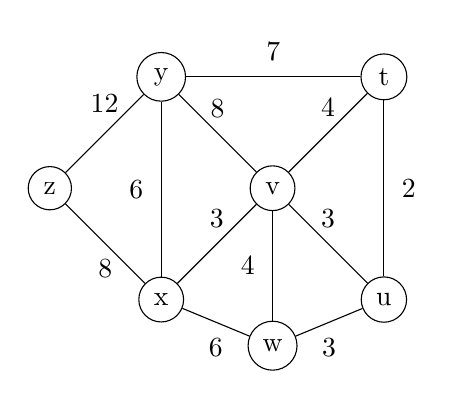
\begin{tikzpicture}
            \tikzstyle{every node} = [align=center, draw, circle, node distance = 2cm]
            \node(v){v};
            \node[below of=v](w){w};
            \node[above right of=v](t){t};
            \node[above left of=v](y){y};
            \node[below right of=v](u){u};
            \node[below left of=v](x){x};
            \node[below left of=y](z){z};

            \path (v) edge node[left, draw=none](){4} (w);
            \path (v) edge node[above, draw=none](){3} (u);
            \path (v) edge node[above, draw=none](){4} (t);
            \path (v) edge node[above, draw=none](){8} (y);
            \path (v) edge node[above, draw=none](){3} (x);

            \path (z) edge node[above, draw=none](){12} (y);
            \path (z) edge node[below, draw=none](){8} (x);

            \path (u) edge node[below, draw=none](){3} (w);
            \path (t) edge node[right, draw=none](){2} (u);
            \path (y) edge node[above, draw=none](){7} (t);
            \path (x) edge node[left, draw=none](){6} (y);
            \path (w) edge node[below, draw=none](){6} (x);
      \end{tikzpicture}
      \caption{A seven node network with given link costs.}
\end{figure}

\subsection*{Solution}

\begin{table}[H]
      \centering
      \begin{tabular}{llllllll}
            Iteration & N'      & y               & z               & w               & u               & v               & t               \\
            1         & x       & (6, x)          & (8, x)          & (6, x)          & $\infty$        & \textbf{(3, x)} & $\infty$        \\
            2         & xv      & \textbf{(6, x)} & (8, x)          & (6, x)          & (6, v)          &                 & (7, v)          \\
            3         & xvy     &                 & (8, x)          & \textbf{(6, x)} & (6, v)          &                 & (7, v)          \\
            4         & xvyw    &                 & (8, x)          &                 & \textbf{(6, v)} &                 & (7, v)          \\
            5         & xvywu   &                 & (8, x)          &                 &                 &                 & \textbf{(7, v)} \\
            5         & xvywuv  &                 & \textbf{(8, x)} &                 &                 &                 &                 \\
            5         & xvywuvz &                 &                 &                 &                 &                 &                 \\
      \end{tabular}
      \caption{
            ``$\infty$'': infinity length, as the actual min length is not known yet.
      }
\end{table}